\documentclass[a4paper,11pt]{article}
\usepackage[T1]{fontenc}

%opening
\title{\texttt{fcc\_tools}\\ a set of tools to facilitate input generation and analysis of FCclasses}
\date{\textsc{Version: 0.1}\\\today}
\author{Javier Cerezo\\\href{mailto:javier.cerezo@uam.es}{\texttt{javier.cerezo@uam.es}}}

% Margins
\textheight 22.0cm \textwidth 14.7cm \oddsidemargin 1cm
\evensidemargin 1cm \topmargin -0.25cm

%Packages
\usepackage{graphics}
\usepackage[pdftex]{graphicx}

\usepackage{amsmath}
\usepackage{amssymb}
\usepackage{color}
\usepackage{xcolor}

\usepackage{hyperref}
% The following metadata will show up in the PDF properties
\hypersetup{
  colorlinks = true,
  urlcolor = blue,
}


\begin{document}
\setlength{\parskip}{0.5em}
\newcommand{\fcc}{$\mathcal{FC}$\textit{classes}}
\newcommand{\fccIII}{$\mathcal{FC}$\textit{classes3}}

\maketitle

\section{Description}
\texttt{fcc\_tools} package provide programs to generate the required data files to run the code from the output of different QM progrms. It also includes some post-processing tools, e.g. to modifiy the broadening scheme, and for analysis. Note that the specific tool to analyze the transitions  from TI calculations through a GUI has a specific documentation.

\section{Installation}

The code is compiled using the usual \texttt{./configure} and \texttt{Makefiles} scripts.

% \clearpage

\subsection{Tools to prepare data files}
The code is provided along with a number of tools to facilitate the preparation of the data files (state, electric dipole...) from the output of a number of electronic structure codes. Codes to post-process the final spectra, allowing to change the broadening scheme without the need of re-running \fccIII\ are also provided. Finally, a GUI to analyze the transitions from a TI calculation is included.

\subsubsection{\texttt{gen\_fcc\_state}}

 \begin{itemize}
  \item[] \textit{Description}:

   A code to generate state files (fcc format) from the output of different electronic structure codes, including Gaussian (fchk and log), Molpro, [Open]Molcas, Turbomol, Gamess, Psi4, Orca and QChem. Molecular Mechanics Hessian and gradients from Gromacs can also be used to build the state files.

   \item[] \textit{Usage}: The code is executed from the command-line:

   \texttt{gen\_fcc\_state -i <output-file> [options]}

   Only the name of the file from which to read the data is mandatory, while the rest of the settings (i.e. state file name) are set automatically from the input base name. Other options, e.g., to read some specific data from different files, can also be set. A complete list of options can be printed to screen with \texttt{gen\_fcc\_state -h}. The options are summarized in the following table.

   \begin{tabular}{lll}
    Flag & Description  \\\hline
 \texttt{-i}    & File to read data from     \\
 \texttt{-fts}  & Set file format            \\
 \texttt{-ih}   & File to read Hessian from  \\
 \texttt{-fth}  & Set file format (Hess)     \\
 \texttt{-ig}   & File to read Gradient from \\
 \texttt{-ftg}  & Set file format (Grad)     \\
 \texttt{-ie}   & File to read Energy from   \\
 \texttt{-fte}  & Set file format (Ener)     \\
 \texttt{-im}   & File to read Mass from     \\
 \texttt{-o}    & File to write state to     \\
 \texttt{-filt} & Filter atoms for output    \\
 \texttt{-write-modes} & Print normal modes    \\
 \texttt{-h}    & Print help\\ \hline
 \multicolumn{2}{c}{Old-\fcc\ specific options}  \\\hline
 \texttt{-write-fcc2} & Write old \fcc\ files \\
 \texttt{-ofcc2}& File to write old-style state  to \\
 \texttt{-om}   & File to write masses to    \\
 \texttt{-force-real} & Turn real all imag freqs \\
 \hline
   \end{tabular}


 \end{itemize}



\subsubsection{\texttt{gen\_fcc\_dipfile}}

\begin{itemize}
  \item[] \textit{Description}:

   A code to generate dipole files (\texttt{ELDIP\_FILE} and \texttt{MAGDIP\_FILE}) from the output of different electronic structure codes, including Gaussian (fchk and log), and Psi4. It can also generate \texttt{NAC\_FILE} (for Gaussian only).

   \item[] \textit{Usage}:

   The code is executed from the command-line:

   \texttt{gen\_fcc\_dipfile -i <output-file> [options]}

   Only the name of the file from which to read the data is mandatory, while the rest of the settings are set automatically (e.g., output names generated from the input base name unless otherwise stated). Other options, e.g., to specify the initial and final states if different from those indicated in the data file, can also be set. A complete list of options can be printed to screen with \texttt{gen\_fcc\_dipfile -h}. The options are summarized in the following table.

   \begin{tabular}{lll}
    Flag & Description  \\\hline
 \texttt{-i}    & File to read data from     \\
 \texttt{-ft}   & Set file format            \\
 \texttt{-Si}   & Initial electronic state (root)  \\
 \texttt{-Sf}   & Final electronic state (root)     \\
 \texttt{-oe}   & File to write eldips to     \\
 \texttt{-om}   & File to write magdips to     \\
 \texttt{-on}   & File to write NACs to   \\
 \texttt{-filt} & Filter atoms for output    \\
 \texttt{-der}  & Read and write tr dipole derivatives    \\
 \texttt{-nac}  & Read and write NACs \\
 \texttt{-h}    & Print help\\ \hline
 \hline
   \end{tabular}


 \end{itemize}


\subsection{Post-calculations tools}
\subsubsection{\texttt{reconvolute\_TD}}

\begin{itemize}
  \item[] \textit{Description}:

   A code to regenerate the spectrum from the correlation function re-adjusting the broadening function  (type and width).

   \item[] \textit{Usage}:

   The code is executed from the command-line:

   \texttt{reconvolute\_TD -hwhm <HWHM> -fccout fcc.out}

   The code must be run on the folder where a TD spectrum calculation has been carried out with \fccIII. It uses some of the files generated in the run (namely \texttt{corr.dat}) along with information included in the output file (since \fccIII\ applies a shift to reduce the computational cost of the TD calculation). The name of the \fccIII\ output will be guessed as \texttt{fcc.out}, but it can be set, along with the value of the new HWHM. Other options, e.g. the type of broadening function, can also be specified. A complete list of options can be printed to screen with \texttt{reconvolute\_TD -h}. The options are summarized in the following table.

   \begin{tabular}{lll}
    Flag & Description  \\\hline
 \texttt{-f}    & File with correlation function    \\
 \texttt{-brd}  & Type of broadening function (Gau,Lor,Voi)            \\
 \texttt{-hwhm} & Width as HWHM in eV  \\
 \texttt{-damp} & Add a damping function to avoid numerical issues     \\
 \texttt{-prop} & Property computed in the \fccIII\ run   \\
 \texttt{-Eshift}& Shift to be applied      \\
 \texttt{-fccout}& File to read shift from   \\
 \texttt{-h}    & Print help\\ \hline
 \hline
   \end{tabular}

 \end{itemize}


\subsubsection{\texttt{reconvolute\_TI}}

\begin{itemize}
  \item[] \textit{Description}:

   A code to regenerate the spectrum from the binned spectrum re-adjusting the broadening function  (type and width).

   \item[] \textit{Usage}:

   The code is executed from the command-line:

   \texttt{reconvolute\_TI -hwhm <HWHM>}

   The code must be run on the folder where a TI spectrum calculation has been carried out with \fccIII. It uses some of the files generated in the run (namely \texttt{Bin\_Spectrum.dat}). The value of the new HWHM is set from the command line. Other options, e.g. the type of broadening function, can also be specified. Note that this tool allows a Voight convolution of the data, which is not still available within the \fccIII\ code for TI calculations. A complete list of options can be printed to screen with \texttt{reconvolute\_TI -h}. The options are summarized in the following table.

   \begin{tabular}{lll}
    Flag & Description  \\\hline
 \texttt{-f}    & File with correlation function    \\
 \texttt{-brd}  & Type of broadening function (Gau,Lor,Voi)            \\
 \texttt{-hwhm} & Width as HWHM in eV  \\
 \texttt{-prop} & Property computed in the \fccIII\ run   \\
 \texttt{-Eshift}& Shift to be applied      \\
 \texttt{-h}    & Print help\\ \hline
 \hline
   \end{tabular}

 \end{itemize}


\subsubsection{\texttt{convolute\_RR}}
\label{S:convolute_RR}

\begin{itemize}
  \item[] \textit{Description}:

   A code to generate the RR spectrum from the 1D or 2D file spectrum adjusting the broadening function (type and width).

   \item[] \textit{Usage}:

   The code is executed from the command-line:

   \texttt{convolute\_RR -type [1D|2D] -hwhm <HWHM>}

   The code must be run on the folder where a RR spectrum calculation has been carried out with \fccIII\ either TD or TI). It uses some of the files generated in the run, namely \texttt{RR\_Spectrum\_VertE.dat} (default for \texttt{-type 1D}) or \texttt{RR\_Spectrum\_2D.dat} (for \texttt{-type 2D}). The value of the new HWHM is set from the command line. When reading the 2D spectrum file, the incident frequency is given on input (\texttt{-wI} flag). The programs looks for the closest value from those included in the 2D file. Other options, e.g. the type of broadening function, can also be specified. A complete list of options can be printed to screen with \texttt{convolute\_RR -h}. The options are summarized in the following table.

   \begin{tabular}{lll}
    Flag & Description  \\\hline
 \texttt{-f}    & File with correlation function    \\
 \texttt{-brd}  & Type of broadening function (Gau,Lor)            \\
 \texttt{-hwhm} & Width as HWHM in cm$^{-1}$  \\
 \texttt{-resol}& Resolution of spectrum in cm$^{-1}$  \\
 \texttt{-type} & Type of output file (1D or 2D)   \\
 \texttt{-wI}   & Selected incident freq (for 2D)     \\
 \texttt{-h}    & Print help\\ \hline
 \hline
   \end{tabular}

 \end{itemize}

\subsection{Analysis tools}
\subsubsection{\texttt{fcc\_analyzer\_PyQt5.py}}
\begin{itemize}
 \item[] \textit{Description}:
 A graphical application to analyze the output of a TI calculation. Graphical interface is build with PyQt5 library. It is a single file script and requires Python3, with packages \texttt{numpy}, \texttt{matplotlib} and \texttt{PyQt5}. It includes the identification of the transitions in terms of the initial and final vibrational states, comparison with experiment or adjustment of the convolution. A brief description of the graphical elements is included in Figure \ref{F:fcc_analyzer}. For a detailed description of the capabilities of the code, consult the specific manual\footnote{\href{https://github.com/jcerezochem/fcc_tools/raw/master/doc/fcc_analyzer_PyQt5_man.pdf}{\texttt{https://github.com/jcerezochem/fcc\_tools/raw/master/doc/fcc\_analyzer\_PyQt5\_man.pdf}}}. The application supports OPA, EMI, ECD, CPL, MCD, TPA and TPCD spectroscopies.
\end{itemize}


\begin{figure}[h!]
\begin{center}
 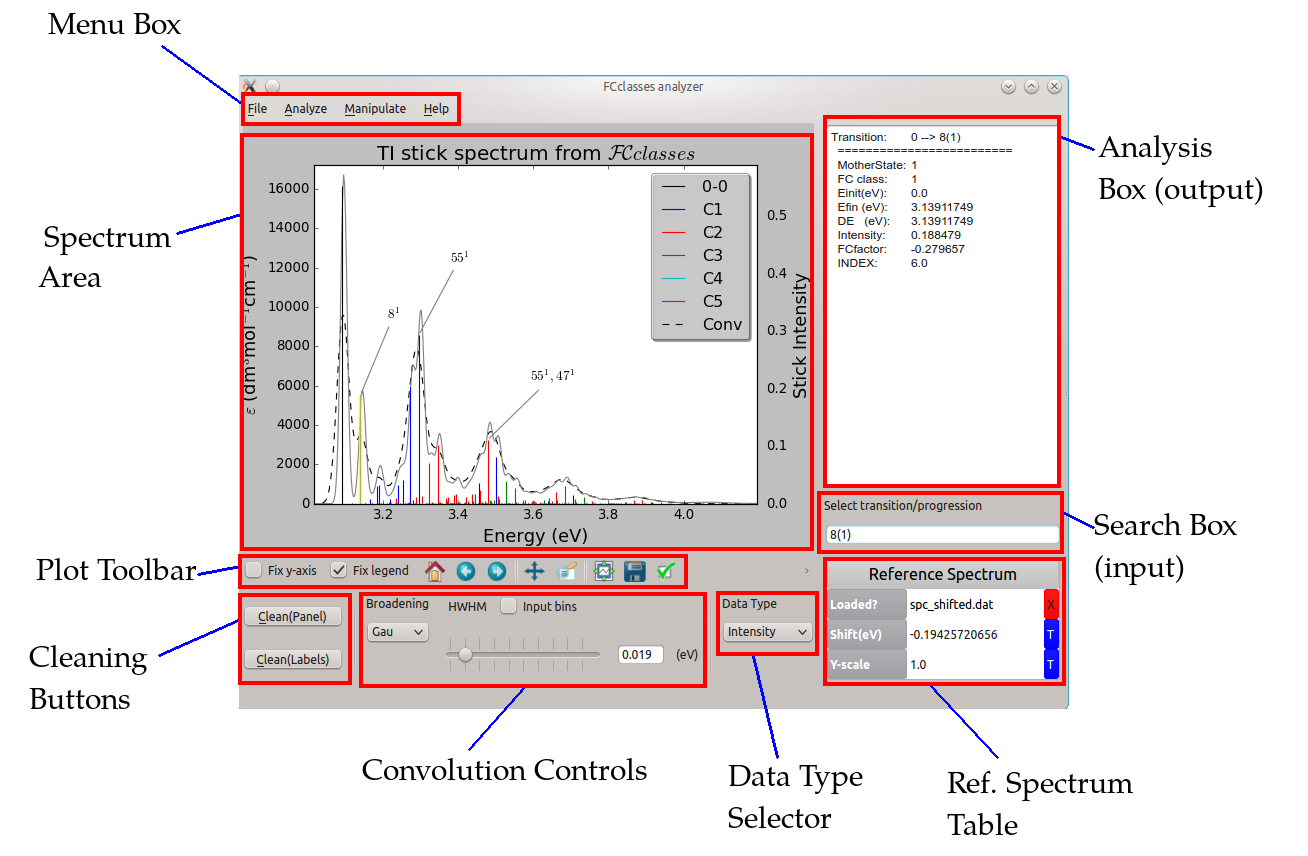
\includegraphics[width=15cm]{figs/fcc_analyzer_screeshot.png}
\end{center}
 \caption{Screenshot of the GUI to analyze TI results.}
\label{F:fcc_analyzer}
\end{figure}

\subsubsection{\texttt{fcc\_RRinspector\_PyQt5.py}}
\begin{itemize}
 \item[] \textit{Description}:
 A graphical application visualize RR spectra, from \texttt{RR\_Spectrum\_2D.dat}. It allows to change the convolution of the RR spectrum (not the damping factor to compute the transtions polarizability) and the indicident frequency.
\end{itemize}


\end{document}
